\clearpage\section{数据与研究方法}

\FloatBarrier\subsection{数据来源}

本文使用的数据集为 FinFE（Financial Forum Emotion），它是中文金融评测基准 BBT-CFLEB 中的情感分类子任务\cite{ref19}。FinFE 的文本来自金融社交媒体上的股民评论，每条评论被标注为消极、中性、积极三类情感之一。与新闻标题、研报等规范文本相比，股民评论篇幅短、口语化程度高，常夹杂股票代码、网络用语和反讽表达，对模型的语义理解能力要求较高。

原论文描述的数据划分为训练集 8000 条、验证集 1000 条、测试集 1000 条，但项目公开仓库中实际提供的文件与之不同：train\_list.json 含 16157 条带标签样本，eval\_list.json 含 2020 条带标签样本，problem\_list.json 含 2020 条无标签样本（排行榜测试集，标签未公开）。由于无标签样本无法用于评估，本文仅使用前两个文件，并以公开文件的实际内容为准重新构建数据集。

\FloatBarrier\subsection{数据质量检查与清洗}

在正式实验前，本文对原始数据进行了质量检查，发现三类问题：

\begin{enumerate}
\def\labelenumi{\arabic{enumi}.}
\tightlist
\item
  训练文件中存在大量重复文本，其中 773 条文本在不同位置被标注为不同标签（标签冲突）；
\item
  原始 eval\_list 的 2020 条记录中，有 1097 条规范化文本也出现在原始训练文件中。原始训练文件随后还会划出验证集，因此这首先说明开发数据与评估数据存在重叠，实际训练曝光与验证曝光需另行区分；
\item
  在分别完成文件内去重、去冲突后，两文件仍有 1092 个重叠文本，其中 228 个跨文件标签不同，说明部分记录的标签存在分歧。
\end{enumerate}

针对这些问题，本文制定了如下清洗规则，并固定随机种子为 42，保证结果可复现：

\begin{enumerate}
\def\labelenumi{\arabic{enumi}.}
\tightlist
\item
  对文本做 Unicode NFKC 规范化，并去除首尾空白字符；
\item
  同一文件内的重复文本，若标签一致则只保留一条，若标签冲突则整组删除；
\item
  以 eval\_list 作为测试集来源，删除其中与训练文件标签不一致的 228 条样本；
\item
  从训练池中删除与文件内清洗后的评估集合重叠的全部文本，包括随后从测试集剔除的 228 个跨文件冲突文本，排除规范化后完全相同文本的跨集合重叠；
\item
  对剩余训练数据按类别分层抽样，划出 10\% 作为验证集，用于超参数选择和早停。
\end{enumerate}

清洗过程各步骤的样本数量变化见表~\ref{tab:3-1}。

\begin{table}[htbp]
\centering
\begin{minipage}{\textwidth}
\setlength{\tabcolsep}{3pt}
\renewcommand{\arraystretch}{1.16}
\setstretch{1.0}\fontsize{10.5}{13.5}\selectfont
\caption{数据清洗过程}\label{tab:3-1}
\begin{tabular}{>{\raggedright\arraybackslash}p{\dimexpr 0.780000\linewidth-3.120000\tabcolsep\relax}>{\raggedright\arraybackslash}p{\dimexpr 0.220000\linewidth-0.880000\tabcolsep\relax}}
\toprule
\textbf{步骤} & \textbf{数量} \\
\midrule
原始训练文件 train\_\allowbreak{}list & 16157 \\
原始评估文件 eval\_\allowbreak{}list & 2020 \\
训练文件：删除重复样本（标签一致） & 3725 \\
训练文件：删除标签冲突的文本 & 773 \\
评估文件：删除重复样本（标签一致） & 61 \\
评估文件：删除标签冲突的文本 & 9 \\
评估文件中与训练文件重复但标签不同的文本（从测试集删除） & 228 \\
训练文件内清洗后与评估集合重叠的文本（含 228 个跨文件冲突文本，均删除） & 1092 \\
\bottomrule\end{tabular}
\end{minipage}
\end{table}

清洗后最终得到训练集 8802 条、验证集 979 条、测试集 1713 条，各数据集的类别分布见表~\ref{tab:3-2} 和图~\ref{fig:3-1}。

\begin{table}[htbp]
\centering
\begin{minipage}{\textwidth}
\setlength{\tabcolsep}{3pt}
\renewcommand{\arraystretch}{1.16}
\setstretch{1.0}\fontsize{10.5}{13.5}\selectfont
\caption{清洗后各数据集类别分布}\label{tab:3-2}
\begin{tabular}{>{\raggedright\arraybackslash}p{\dimexpr 0.200000\linewidth-2.000000\tabcolsep\relax}>{\raggedright\arraybackslash}p{\dimexpr 0.200000\linewidth-2.000000\tabcolsep\relax}>{\raggedright\arraybackslash}p{\dimexpr 0.200000\linewidth-2.000000\tabcolsep\relax}>{\raggedright\arraybackslash}p{\dimexpr 0.200000\linewidth-2.000000\tabcolsep\relax}>{\raggedright\arraybackslash}p{\dimexpr 0.200000\linewidth-2.000000\tabcolsep\relax}}
\toprule
\textbf{数据集} & \textbf{消极} & \textbf{中性} & \textbf{积极} & \textbf{合计} \\
\midrule
训练集 & 2044（23.2\%） & 1845（21.0\%） & 4913（55.8\%） & 8802 \\
验证集 & 227（23.2\%） & 205（20.9\%） & 547（55.9\%） & 979 \\
测试集 & 461（26.9\%） & 438（25.6\%） & 814（47.5\%） & 1713 \\
\bottomrule\end{tabular}
\end{minipage}
\end{table}

\begin{figure}[htbp]\centering
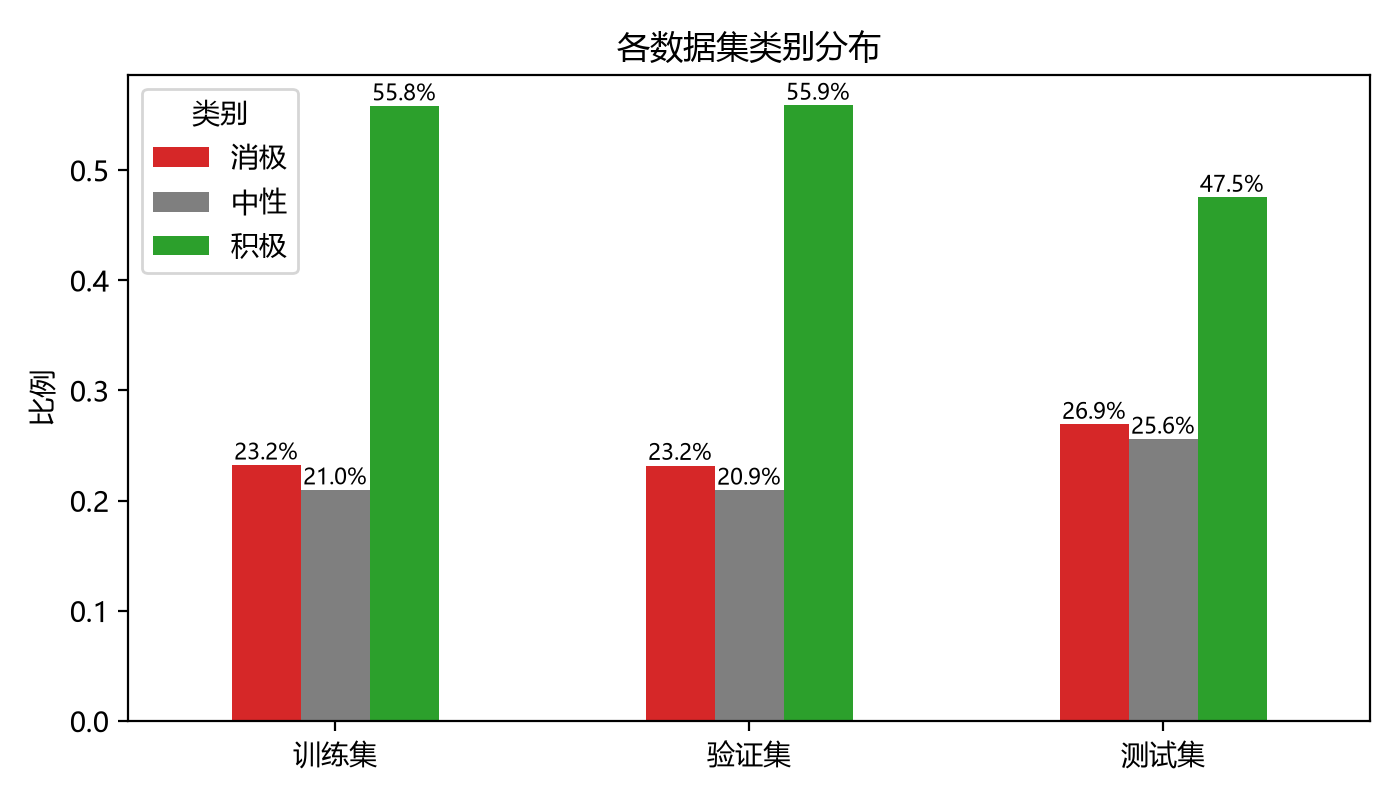
\includegraphics[width=\linewidth,height=0.80\textheight,keepaspectratio]{figures/fig_label_dist.png}
\caption{各数据集类别分布}\label{fig:3-1}\end{figure}

对``数据集 \(\times\) 类别''列联表做卡方检验，得到 \(\chi^{2}\) = 41.09，自由度为 4，p = 2.6\(\times\)10\(^{-8}\)，说明测试集的类别比例与训练集存在显著差异：测试集中积极类占比较低，消极类和中性类占比较高。该差异与去重、冲突删除及重新划分后的样本构成有关，不能单独归因于去除泄露。由于类别分布不均衡，且训练集与测试集分布不完全一致，本文以宏平均 F1 值（Macro-F1）作为主要评价指标，准确率作为辅助指标。依据跨文件标签一致性删除评估记录会改变评估对象，可能排除更难或更有歧义的样本；因此后续结论限于该清洗规则下的数据，不能视为对原始评论总体的无偏估计。本文也未系统排除近重复和预训练数据污染。

\FloatBarrier\subsection{描述性统计分析}

\subsubsection{文本长度}

FinFE 文本整体很短，各类别的长度统计见表~\ref{tab:3-3}。积极类评论平均长度为 22.6 个字符，明显长于消极类（19.6）和中性类（19.7）。由于长度分布明显右偏（见图~\ref{fig:3-2}），本文采用非参数的 Kruskal-Wallis 检验比较三类文本的长度分布，结果为 H = 157.21，p = 7.3\(\times\)10\(^{-35}\)，差异极显著。这说明文本长度本身携带一定的情感信息，但三类之间的长度分布重叠很大，仅靠长度无法有效区分情感。

\begin{table}[htbp]
\centering
\begin{minipage}{\textwidth}
\setlength{\tabcolsep}{3pt}
\renewcommand{\arraystretch}{1.16}
\setstretch{1.0}\fontsize{10.5}{13.5}\selectfont
\caption{各类别文本长度（字符）}\label{tab:3-3}
\begin{tabular}{>{\raggedright\arraybackslash}p{\dimexpr 0.142857\linewidth-2.000000\tabcolsep\relax}>{\raggedright\arraybackslash}p{\dimexpr 0.142857\linewidth-2.000000\tabcolsep\relax}>{\raggedright\arraybackslash}p{\dimexpr 0.142857\linewidth-2.000000\tabcolsep\relax}>{\raggedright\arraybackslash}p{\dimexpr 0.142857\linewidth-2.000000\tabcolsep\relax}>{\raggedright\arraybackslash}p{\dimexpr 0.142857\linewidth-2.000000\tabcolsep\relax}>{\raggedright\arraybackslash}p{\dimexpr 0.142857\linewidth-2.000000\tabcolsep\relax}>{\raggedright\arraybackslash}p{\dimexpr 0.142857\linewidth-2.000000\tabcolsep\relax}}
\toprule
\textbf{类别} & \textbf{样本数} & \textbf{均值} & \textbf{标准差} & \textbf{最小值} & \textbf{中位数} & \textbf{最大值} \\
\midrule
消极 & 2732 & 19.62 & 13.57 & 4 & 16 & 66 \\
中性 & 2488 & 19.72 & 13.64 & 4 & 16 & 67 \\
积极 & 6274 & 22.56 & 14.26 & 4 & 19 & 68 \\
\bottomrule\end{tabular}
\end{minipage}
\end{table}

\begin{figure}[htbp]\centering
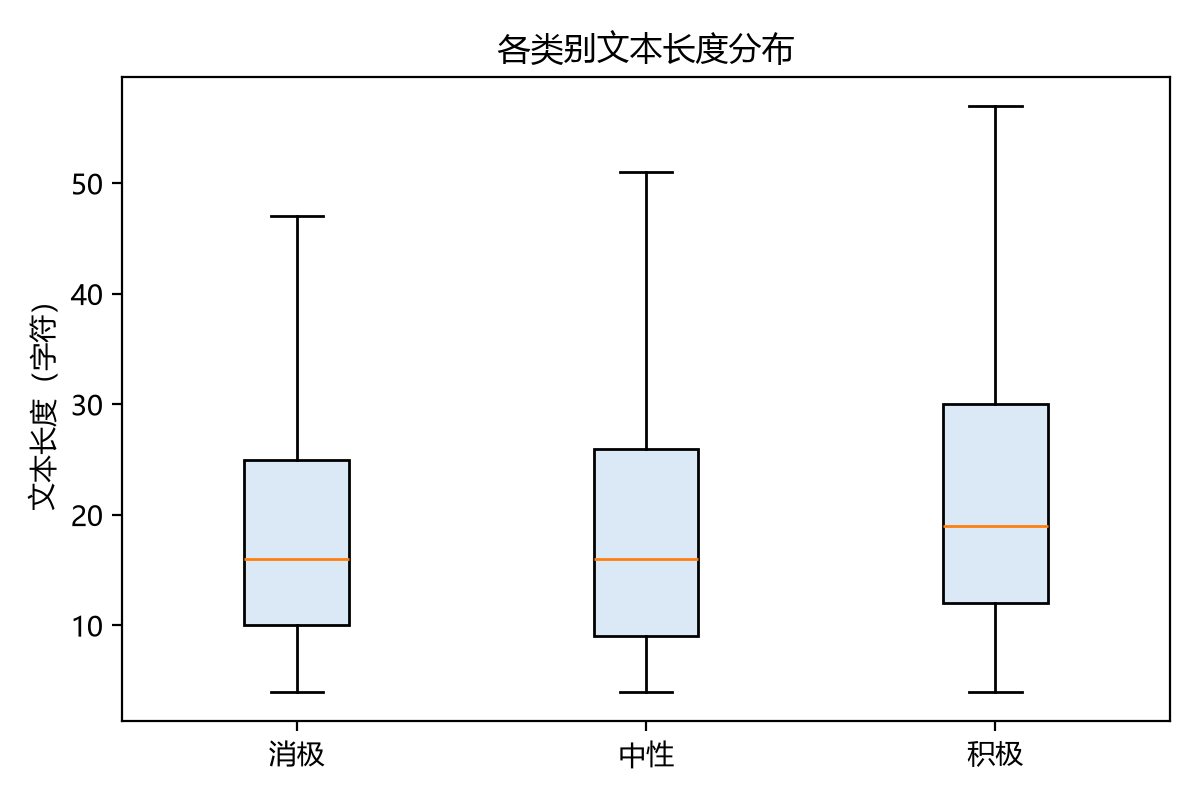
\includegraphics[width=\linewidth,height=0.80\textheight,keepaspectratio]{figures/fig_length_by_label.png}
\caption{各类别文本长度分布}\label{fig:3-2}\end{figure}

\subsubsection{文本特征}

本文进一步统计了否定词、数字、问号和感叹号四类表层特征在各类别中的出现比例，并对每个特征做卡方独立性检验，结果见表~\ref{tab:3-4}。四个特征与情感类别均显著相关（p 均小于 10\(^{-23}\)）：消极类评论更常出现否定词（40.2\%），中性类评论更常出现问号（17.8\%，多为向其他股民提问），积极类评论更常出现感叹号（20.9\%）和数字。中性类的问句特征提示，这一类别中有相当部分评论并不表达明确态度，这可能是后文各模型在中性类上表现最差的原因之一。

\begin{table}[htbp]
\centering
\begin{minipage}{\textwidth}
\setlength{\tabcolsep}{3pt}
\renewcommand{\arraystretch}{1.16}
\setstretch{1.0}\fontsize{10.5}{13.5}\selectfont
\caption{文本特征在各类别中的占比}\label{tab:3-4}
\begin{tabular}{>{\raggedright\arraybackslash}p{\dimexpr 0.166667\linewidth-2.000000\tabcolsep\relax}>{\raggedright\arraybackslash}p{\dimexpr 0.166667\linewidth-2.000000\tabcolsep\relax}>{\raggedright\arraybackslash}p{\dimexpr 0.166667\linewidth-2.000000\tabcolsep\relax}>{\raggedright\arraybackslash}p{\dimexpr 0.166667\linewidth-2.000000\tabcolsep\relax}>{\raggedright\arraybackslash}p{\dimexpr 0.166667\linewidth-2.000000\tabcolsep\relax}>{\raggedright\arraybackslash}p{\dimexpr 0.166667\linewidth-2.000000\tabcolsep\relax}}
\toprule
\textbf{特征} & \textbf{消极} & \textbf{中性} & \textbf{积极} & \textbf{$\chi^{2}$} & \textbf{p} \\
\midrule
含否定词 & 40.2\% & 33.3\% & 29.1\% & 107.352 & 4.9$\times$10$^{-24}$ \\
含数字 & 19.8\% & 27.7\% & 30.5\% & 108.565 & 2.7$\times$10$^{-24}$ \\
含问号 & 8.8\% & 17.8\% & 4.5\% & 408.784 & 1.7$\times$10$^{-89}$ \\
含感叹号 & 15.4\% & 10.8\% & 20.9\% & 135.512 & 3.7$\times$10$^{-30}$ \\
\bottomrule\end{tabular}
\end{minipage}
\end{table}

\subsubsection{高频词}

使用 jieba 分词并去除停用词后，训练集各类别的高频词见图~\ref{fig:3-3}。消极类的高频词包括``垃圾''\,``下跌''\,``跌停''\,``大跌''\,``出货''\,``退市''，积极类包括``涨停''\,``加油''\,``加仓''\,``买入''\,``看好''\,``龙头''，均符合股民的表达习惯。中性类的高频词如``看看''\,``一下''\,``多少''\,``可能''，大多不带情感倾向，进一步印证了中性类以提问和陈述为主的特点。

\begin{figure}[htbp]\centering
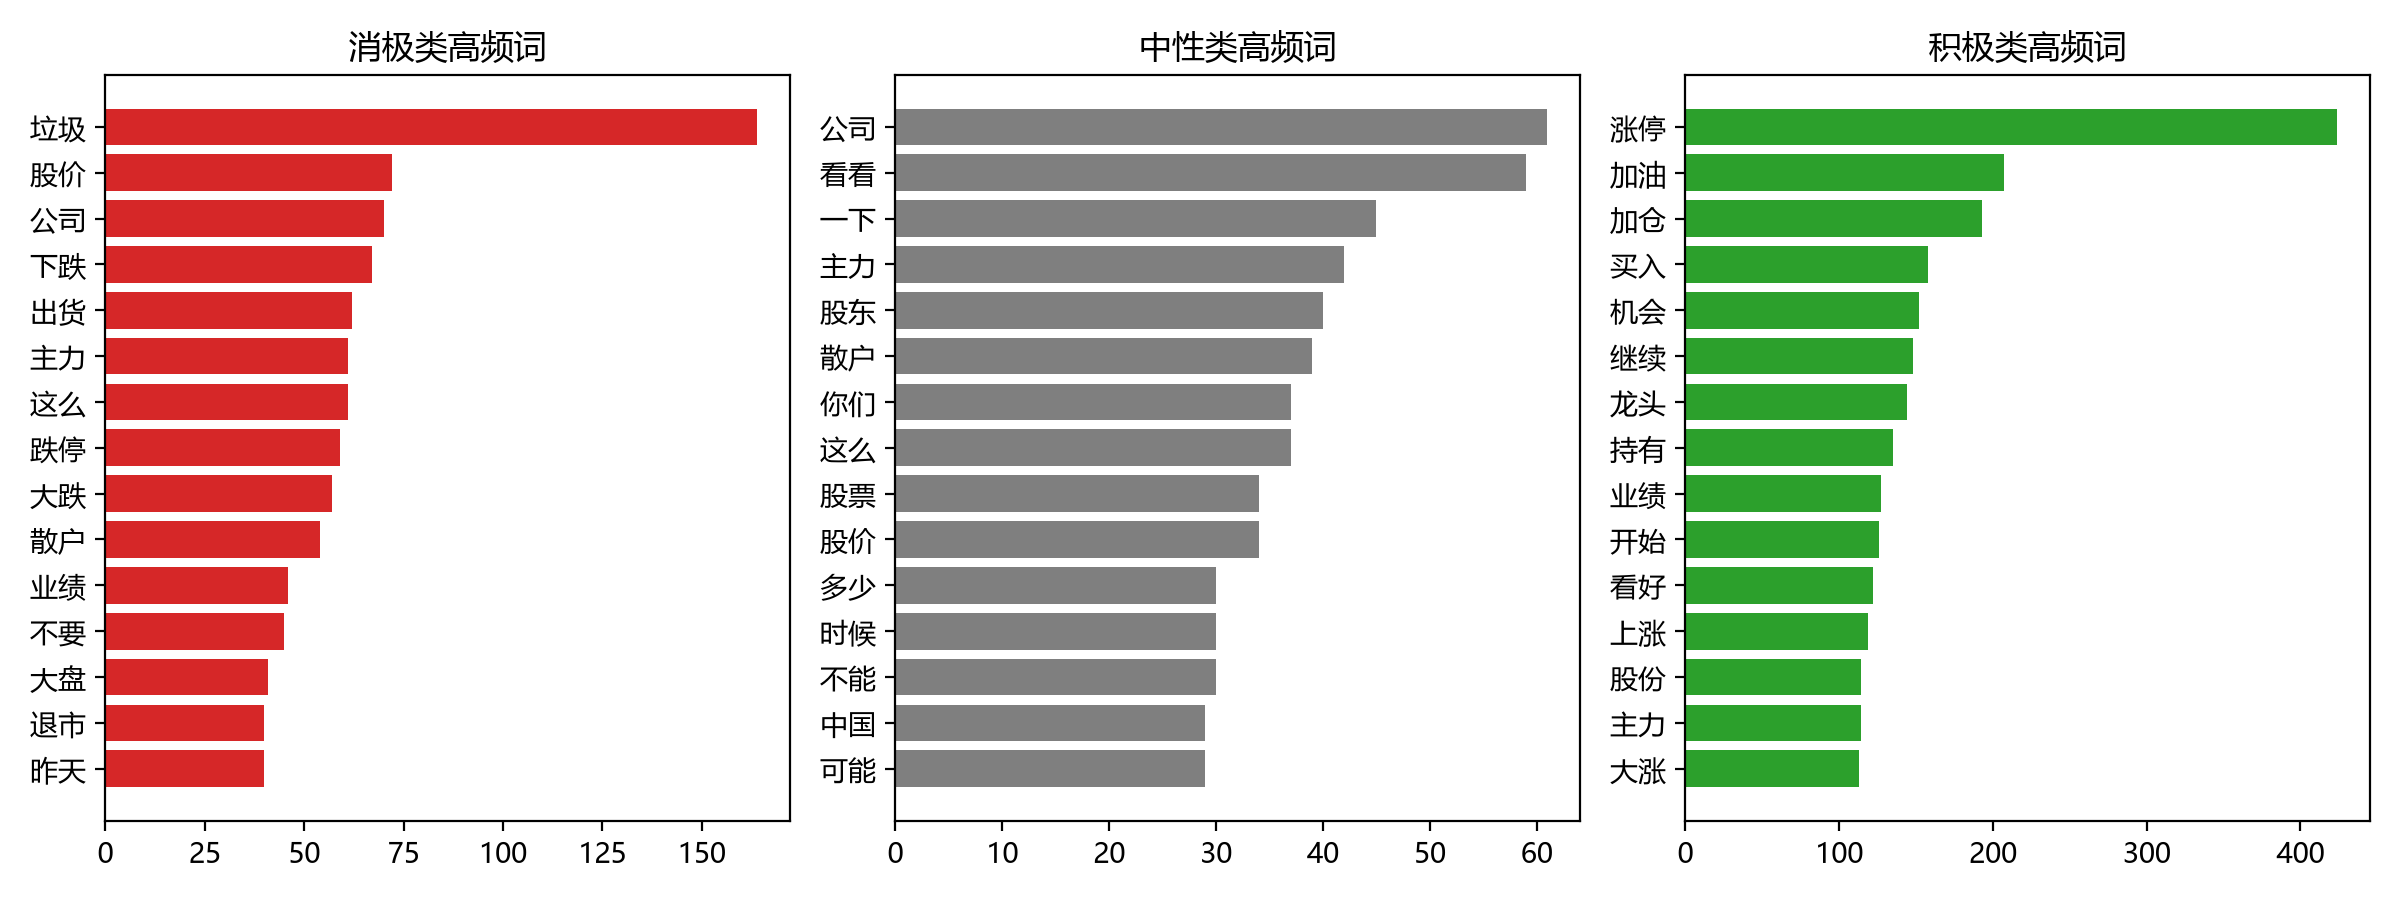
\includegraphics[width=\linewidth,height=0.80\textheight,keepaspectratio]{figures/fig_top_words.png}
\caption{训练集各类别高频词}\label{fig:3-3}\end{figure}

\FloatBarrier\subsection{对比模型}

为全面评估大语言模型的效果，本文设置了四类模型，见表~\ref{tab:3-5}。

\begin{table}[htbp]
\centering
\begin{minipage}{\textwidth}
\setlength{\tabcolsep}{3pt}
\renewcommand{\arraystretch}{1.16}
\setstretch{1.0}\fontsize{10.5}{13.5}\selectfont
\caption{实验模型}\label{tab:3-5}
\begin{tabular}{>{\raggedright\arraybackslash}p{\dimexpr 0.190000\linewidth-1.520000\tabcolsep\relax}>{\raggedright\arraybackslash}p{\dimexpr 0.400000\linewidth-3.200000\tabcolsep\relax}>{\raggedright\arraybackslash}p{\dimexpr 0.130000\linewidth-1.040000\tabcolsep\relax}>{\raggedright\arraybackslash}p{\dimexpr 0.280000\linewidth-2.240000\tabcolsep\relax}}
\toprule
\textbf{类别} & \textbf{模型} & \textbf{参数量} & \textbf{使用方式} \\
\midrule
传统机器学习 & TF-\allowbreak{}IDF + 逻辑回归 /\allowbreak{} 线性 SVM & — & 有监督训练 \\
预训练语言模型 & BERT-\allowbreak{}base-\allowbreak{}Chinese\cite{ref7} & 1.0 亿 & 全参数微调 \\
预训练语言模型 & Chinese-\allowbreak{}RoBERTa-\allowbreak{}wwm-\allowbreak{}ext\cite{ref9} & 1.0 亿 & 全参数微调 \\
大语言模型 & Qwen3-\allowbreak{}8B、Qwen2.5-\allowbreak{}7B-\allowbreak{}Instruct、GLM-\allowbreak{}4-\allowbreak{}9B-\allowbreak{}Chat & 70 亿～94 亿 & 零样本、少样本提示；LoRA 微调 \\
\bottomrule\end{tabular}
\end{minipage}
\end{table}

传统基线采用字符级 1～3 元组的 TF-IDF 特征，分类器的正则化系数 C 在验证集上从 \{0.1, 0.3, 1, 3, 10, 30, 100\} 中选择。线性 SVM 本身不输出概率，本文用 sigmoid 校准（5 折交叉验证）得到三类概率，以便与其他模型统一做校准分析。

预训练语言模型采用标准的序列分类微调：学习率 2\(\times\)10\(^{-5}\)，批大小 32，最多训练 5 轮，前 10\% 步数线性预热后线性衰减，最大序列长度 96，以验证集 Macro-F1 早停（连续 2 轮不提升即停止）。

\FloatBarrier\subsection{大语言模型的分类方法}

\subsubsection{提示设计}

本文将情感分类表述为对话任务。系统提示为``你是一名金融文本情感分析助手。''，用户提示为：

\begin{quote}\small 请判断下面这条股民评论的情感倾向，只能回答“消极”“中性”“积极”三者之一，不要输出其他内容。\par 评论：\{评论文本\}\end{quote}

提示经各模型自带的对话模板渲染后输入模型。对于 Qwen3-8B，本文关闭了其``思考模式''，使模型直接给出答案。少样本设置下，从训练集中每类随机抽取 k 条样本（k = 1 或 3，随机种子 42），以``用户提问---助手回答''的多轮对话形式放在待测评论之前。

\subsubsection{基于标签词的概率提取}

采用第 2 章式（2-5）的标签词方法：读取答案首位置对``消极''\,``中性''\,``积极''三个标签首 token 的 logit，再在这三个值间归一化。代码断言三个 token ID 互异，预测取最大概率类别。它避免了自由生成后的文本解析，但所得概率依赖提示与标签词，并非完整答案字符串的生成概率。

\subsubsection{LoRA 微调}

本文采用第 2 章式（2-6）的 LoRA 结构。本文在注意力层的 q、k、v、o 投影和前馈层的 gate、up、down 投影上都加入 LoRA 模块，主实验取 r = 16、\(\alpha\) = 32、dropout = 0.05。以 Qwen3-8B 为例，可训练参数为 4365 万，仅占总参数量（82.3 亿）的 0.53\%。

训练时在答案的第一个位置上，对正确标签词首 token 计算全词表交叉熵，而不是对完整标签词序列逐 token 计算损失。推理时再将三个标签首 token 的 logits 归一化为三分类概率，两者共享标签映射，但训练损失的分母是全词表。优化器为 AdamW，学习率 1\(\times\)10\(^{-4}\)，有效批大小 16，训练 2 轮，前 5\% 步数线性预热后线性衰减，梯度裁剪阈值 1.0，采用 bf16 混合精度和梯度检查点以节省显存。每轮结束后在验证集上计算 Macro-F1，保留最优一轮的 LoRA 权重用于测试。

为考察量化对效果的影响，本文还实现了 QLoRA\cite{ref15}：以 4-bit NF4 格式加载冻结的基础模型权重（采用双重量化），计算 dtype 设为 bf16；不将适配器各张量精度与量化基础权重的存储精度混为一谈。

\FloatBarrier\subsection{实验环境与重复设计}

全部实验在一台配备 NVIDIA RTX 3090（24 GB 显存）、32 GB 内存的 Windows 计算机上完成，软件环境为 Python 3.11、PyTorch 2.7.1（CUDA 12.8）、transformers、peft 和 bitsandbytes。

为区分模型差异与训练随机性，BERT、RoBERTa 和三个大模型的 LoRA 微调均使用 3 个随机种子（42、43、44）重复训练。零样本推理是确定性的，只运行一次；少样本和消融实验受计算资源限制，只使用种子 42。

\begin{table}[htbp]
\centering
\begin{minipage}{\textwidth}
\setlength{\tabcolsep}{3pt}
\renewcommand{\arraystretch}{1.16}
\setstretch{1.0}\fontsize{10.5}{13.5}\selectfont
\caption{关键实验配置与核验依据}\label{tab:3-6}
\begin{tabular}{>{\raggedright\arraybackslash}p{\dimexpr 0.190000\linewidth-1.140000\tabcolsep\relax}>{\raggedright\arraybackslash}p{\dimexpr 0.650000\linewidth-3.900000\tabcolsep\relax}>{\raggedright\arraybackslash}p{\dimexpr 0.160000\linewidth-0.960000\tabcolsep\relax}}
\toprule
\textbf{对象} & \textbf{关键设置} & \textbf{核验依据} \\
\midrule
TF-\allowbreak{}IDF 特征 & 字符 1～3 元组；min\_\allowbreak{}df=2；次线性词频、平滑 IDF、L2 归一化 & 实现 I \\
LR /\allowbreak{} SVM & C 候选为 0.1、0.3、1、3、10、30、100；实际选择分别为 10、0.3；类别权重 balanced & 记录 R、实现 I \\
SVM 概率 & 训练数据内 5 折 sigmoid 校准；外部验证集选择 C & 实现 I \\
BERT /\allowbreak{} RoBERTa & 学习率 2$\times$10$^{-5}$；批大小 32；长度上限 96；AdamW 权重衰减 0.01 & 记录 R、实现 I \\
BERT /\allowbreak{} RoBERTa 选择 & 最多 5 轮；预热 10\%；验证 F1 连续 2 轮不提升停止；保留验证最优权重 & 实现 I；实际轮数见注 \\
LoRA 主配置 & r=16，$\alpha$=32，dropout=0.05；q/\allowbreak{}k/\allowbreak{}v/\allowbreak{}o 与 gate/\allowbreak{}up/\allowbreak{}down 七类投影 & 记录 R、实现 I \\
LoRA 优化与选择 & 学习率 1$\times$10$^{-4}$；有效批大小 16；训练 2 轮；AdamW 权重衰减 0；预热 5\%；验证最优轮 & 记录 R、实现 I \\
LLM 输入与损失 & 按模型对话模板、左侧填充；当前代码不主动截断；答案首位置全词表交叉熵；推理在三个标签 token 间归一化 & 实现 I \\
重复与单次实验 & BERT、RoBERTa、三个 LoRA：42 /\allowbreak{} 43 /\allowbreak{} 44；提示与配置消融另按单次口径报告 & 记录 R \\
\bottomrule\end{tabular}
\par\vspace{3pt}{\fontsize{10}{12.5}\selectfont 注：R 指 outputs/\allowbreak{}metrics 中实际运行记录，I 指 src/\allowbreak{}baselines 与 src/\allowbreak{}llm 中当前实现；记录与实现共同核对，不把代码默认值冒称为完整历史参数快照。两类编码器在种子 42、43、44 下实际均运行 4、5、4 轮（不是最佳轮次）。LoRA 记录确认主实验未启用 4-\allowbreak{}bit；4-\allowbreak{}bit 是独立消融。微批量未在历史 metrics 中完整保存，故不补写为已证实的运行参数。\par}
\end{minipage}
\end{table}

\FloatBarrier\subsection{评价指标与统计方法}

\subsubsection{分类指标}

按第 2 章式（2-7）和式（2-8）计算类精确率、召回率、F1 与 Macro-F1，准确率为辅助指标。主结果表区分多种子均值与单次区间，错误分析另行报告种子 42 的混淆矩阵，避免把两种口径混用。

\subsubsection{显著性检验}

\textbf{McNemar 与 Holm 校正。} 使用第 2 章式（2-10）的连续性校正检验；不一致样本总数小于 25 时使用精确二项检验。固定 TF-IDF+LR、RoBERTa 与三个 LoRA 模型构成比较集合，在同一测试集上取种子 42 或单次预测，全部十对 p 值统一作 Holm 校正\cite{ref27,ref29}。

\textbf{配对 Bootstrap。} McNemar 检验针对准确率，而主要指标 Macro-F1 不是逐样本可加的统计量。本文固定种子 42 的模型预测，在同一组有放回抽取的测试样本上计算各模型的 Macro-F1 差值\cite{ref28}。修订分析将差值的重抽样次数增加到 B = 50000，独立固定抽样 RNG 种子为 20261012。先报告单个比较的 95\% 百分位区间，再将 TF-IDF+LR、RoBERTa 和三个 LoRA 模型的全部十对构成一个比较家族，使用 0.25\% 和 99.75\% 分位数作 Bonferroni 调整区间，名义家族覆盖率为 95\%。该调整仍为 Bootstrap 近似，不把未调整区间刚好不含 0 视为稳健的多重比较结论。表~\ref{tab:4-1} 的单模型区间仍使用 B = 2000，并明确其仅对应种子 42 或单次运行。

\textbf{方差分析。} 对使用 3 个随机种子的模型，以各次运行的 Macro-F1 为观测值做单因素方差分析，检验不同模型的平均 Macro-F1 是否相同。先用 Levene 检验检查方差差异，同时报告不要求方差齐性的 Welch 方差分析作为稳健性检验；若整体显著，再用 Tukey HSD 方法做两两事后比较。

上述配对分析条件于已训练模型，多种子分析条件于固定数据划分；两者都不涵盖更换来源或时期后的分布变化。

\subsubsection{校准分析}

按第 2 章式（2-12），以 15 个等宽置信度区间计算 ECE，并报告 MCE、Brier 分数和 NLL\cite{ref22}。它们刻画的性质不同，不根据单个最小值宣称模型整体最可靠。

按第 2 章式（2-13）作温度缩放，以 NLL 拟合 T\cite{ref22}。由于大模型实验只保存了测试集的预测概率，本文在测试集上采用 5 折交叉拟合：在 4 折上估计 T，应用于剩下的 1 折，使每个样本的校准概率来自未使用其自身标签拟合的温度参数。这里评估的是同一测试分布内的交叉拟合效果，不是独立外部测试，也没有得到一个经独立验证的部署温度。

历史预测 CSV 只保存了六位小数概率。本文在 log(p) 和 NLL 计算中将零值截到 1e-12，此约定不能恢复被舍入丢失的尾部精度，尤其影响零样本模型。为此另报告 1e-6、1e-8、1e-12 三种截断下限的敏感性，既不把任一替代值当成真实概率，也不改写历史预测；后续概率保存已改为不预先舍入。

\subsubsection{选择性预测}

在实际应用中，模型可以只对有把握的样本给出判断，对没把握的样本交由人工处理。将测试样本按置信度从高到低排序，只保留前 c 比例的样本作答（c 称为覆盖率），计算这部分样本的错误率（风险），得到风险-覆盖率曲线。曲线下面积 AURC 越小，说明模型的置信度越能区分对错\cite{ref23}。由于 AURC 也受模型整体错误率影响，本文同时报告 E-AURC，即 AURC 减去在同样错误率下按理想排序可达到的最小 AURC，它只衡量置信度排序的质量。

\subsubsection{描述性错误分析}

使用 TF-IDF+LR、RoBERTa 与 Qwen3-8B LoRA 的已有种子 42 预测，逐行核对文本、标签与清洗后测试集完全一致，计算混淆矩阵及类精确率、召回率、F1。Qwen3 作为已有消融对象，用于保持分析对象连贯，不是按本次错误表现选出的最佳模型。

对 Qwen3 的六种有方向误分类分别按 SHA256("error-audit-v1" + 空字符 + 原文) 排序，各取前两条形成 12 条核读材料，正文展示每组第一条。样例保留文本原貌，以数据行号追溯。该分层固定抽样是定性说明，不能估计反讽等错误类型在总体中的占比，也不充当独立复标。脚本与机器可读输出分别保存于 scripts/analyze\_error\_cases.py 和 outputs/analysis/editorial-20261013。
